\section{System overview}

\subsection{Grid configuration}
The HVDC system is a point-to-point, bidirectional VSC-HVDC link connecting the converter stations via a DC
transmission line. An overview of the system with HVDC scope of supply is shown in
Figure~\ref{fig:system-overview-poi1}.

\begin{figure}[htbp]
  \centering
  
\includegraphics[width=\linewidth]{fig/system_overview.pdf}
  \caption{System overview with HVDC system scope of supply}
  \label{fig:system-overview-poi1}
\end{figure}

\subsection{Transmission schemes}
The transmission system will utilize two HVDC schemes. The schemes differ in their power rating, which might result in 
different transmission topologies. An overview of the technical parameters is given in Table~\ref{tab:system-ratings}.

% \begin{center}

\begin{table}[htbp]
  \centering
  % \renewcommand{\arraystretch}{1.3}
  \begin{tabular}{@{}l l l l@{}}
    \toprule
    \multicolumn{1}{@{}c}{\textbf{Parameter}} & \multicolumn{1}{c}{\textbf{Description}} &
    \multicolumn{1}{c}{\textbf{Scheme 1}} & \multicolumn{1}{c@{}}{\textbf{Scheme 2}} \\
    \midrule
    $P_{AC\_Rec}$ & Rated active power (AC inverter) & 3000\,MW & 1000\,MW \\
    $Q_{AC\_Rec}$ & Rated reactive power & $\pm$ 990 MVAr & $\pm$330 MVAr \\
    $U_{DC}$      & Rated DC voltage (pole--ground)   & $\pm$400\,kV, $\pm$525\,kV & $\pm$400\,kV \\
    Config.       & Transmission configuration        & DSMP or BIP with DMR & SMP \\
    $L$           & DC line length                    & $\sim$200\,mi & $\sim$200\,mi \\
    $f$           & AC system frequency               & 60\,Hz & 60\,Hz \\
    \bottomrule
  \end{tabular}
  \caption{HVDC configuration: Scheme 1 and Scheme 2.}
  \label{tab:system-ratings}
\end{table}

For the reactive power an initial power factor of $\cos \phi = 0.95$ was defined. As the system investigations are ongoing,
it is expected that the reactive power requirements can be significantly reduced.

% \end{center}
\pagebreak

\subsection{HVDC topologies}

\subsubsection{Scheme 1}
For the 3000\,MW Scheme~1, two transmission configurations are considered: 
\begin{enumerate}
  \item Dual symmetrical monopole (DSMP, Figure~\ref{fig:config-dsmp}) with $\pm$400\,kV DC voltage
  \item Bipole with dedicated metallic return (BIP, Figure~\ref{fig:config-bip}) with $\pm$525\,kV DC voltage
\end{enumerate}

The DSMP configuration is assumed to provide higher availability and greater flexibility
for the staged buildout of the transmission line. Furthermore, the same converter configuration can be used for Scheme 2, 
taking into account an overrating of the Scheme 2 configuration. The DC voltage of $\pm$400\,kV was selected two allow DC cable sections 
without installation of parallel cables.\\
The DSMP configuration is the preferred topology. The BIP configuration will be used only in case of signigicant DC line price reduction.


\begin{figure}[htbp]
  \centering
  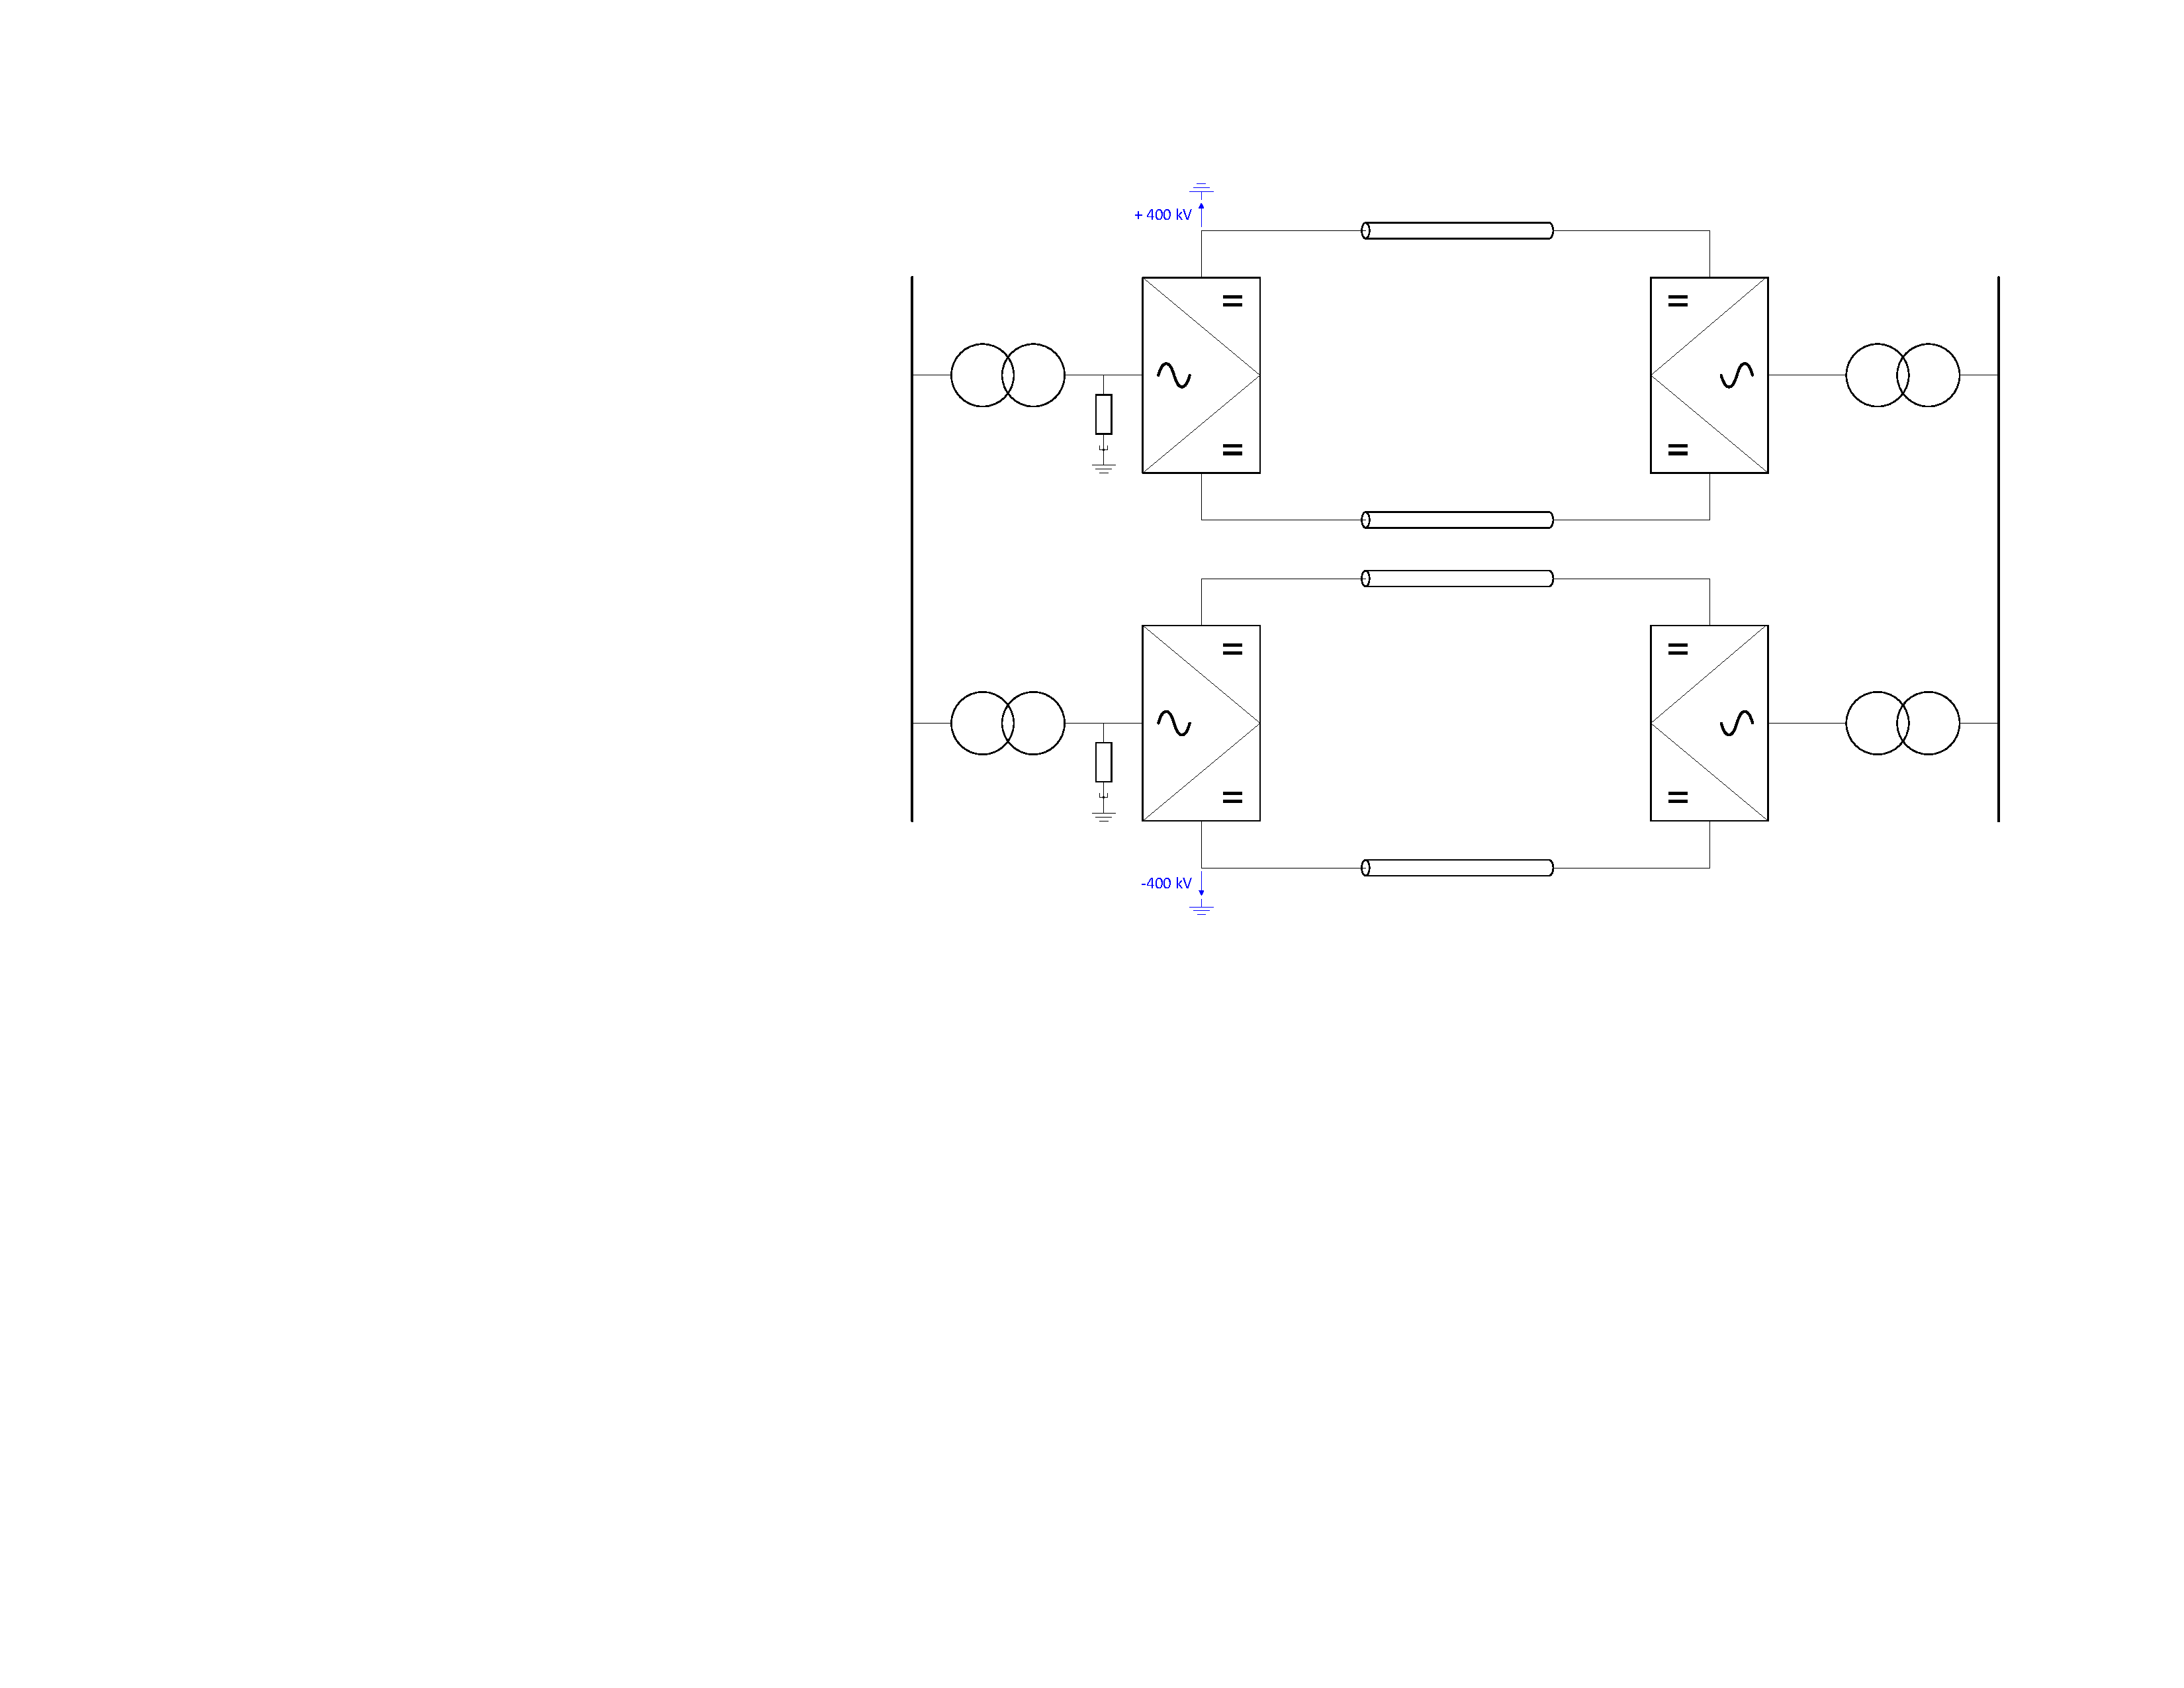
\includegraphics[width=0.7\linewidth]{fig/config_dsmp.pdf}
  \caption{Dual symmetrical monopole (DSMP) configuration.}
  \label{fig:config-dsmp}
\end{figure}

\begin{figure}[htbp]
  \centering
  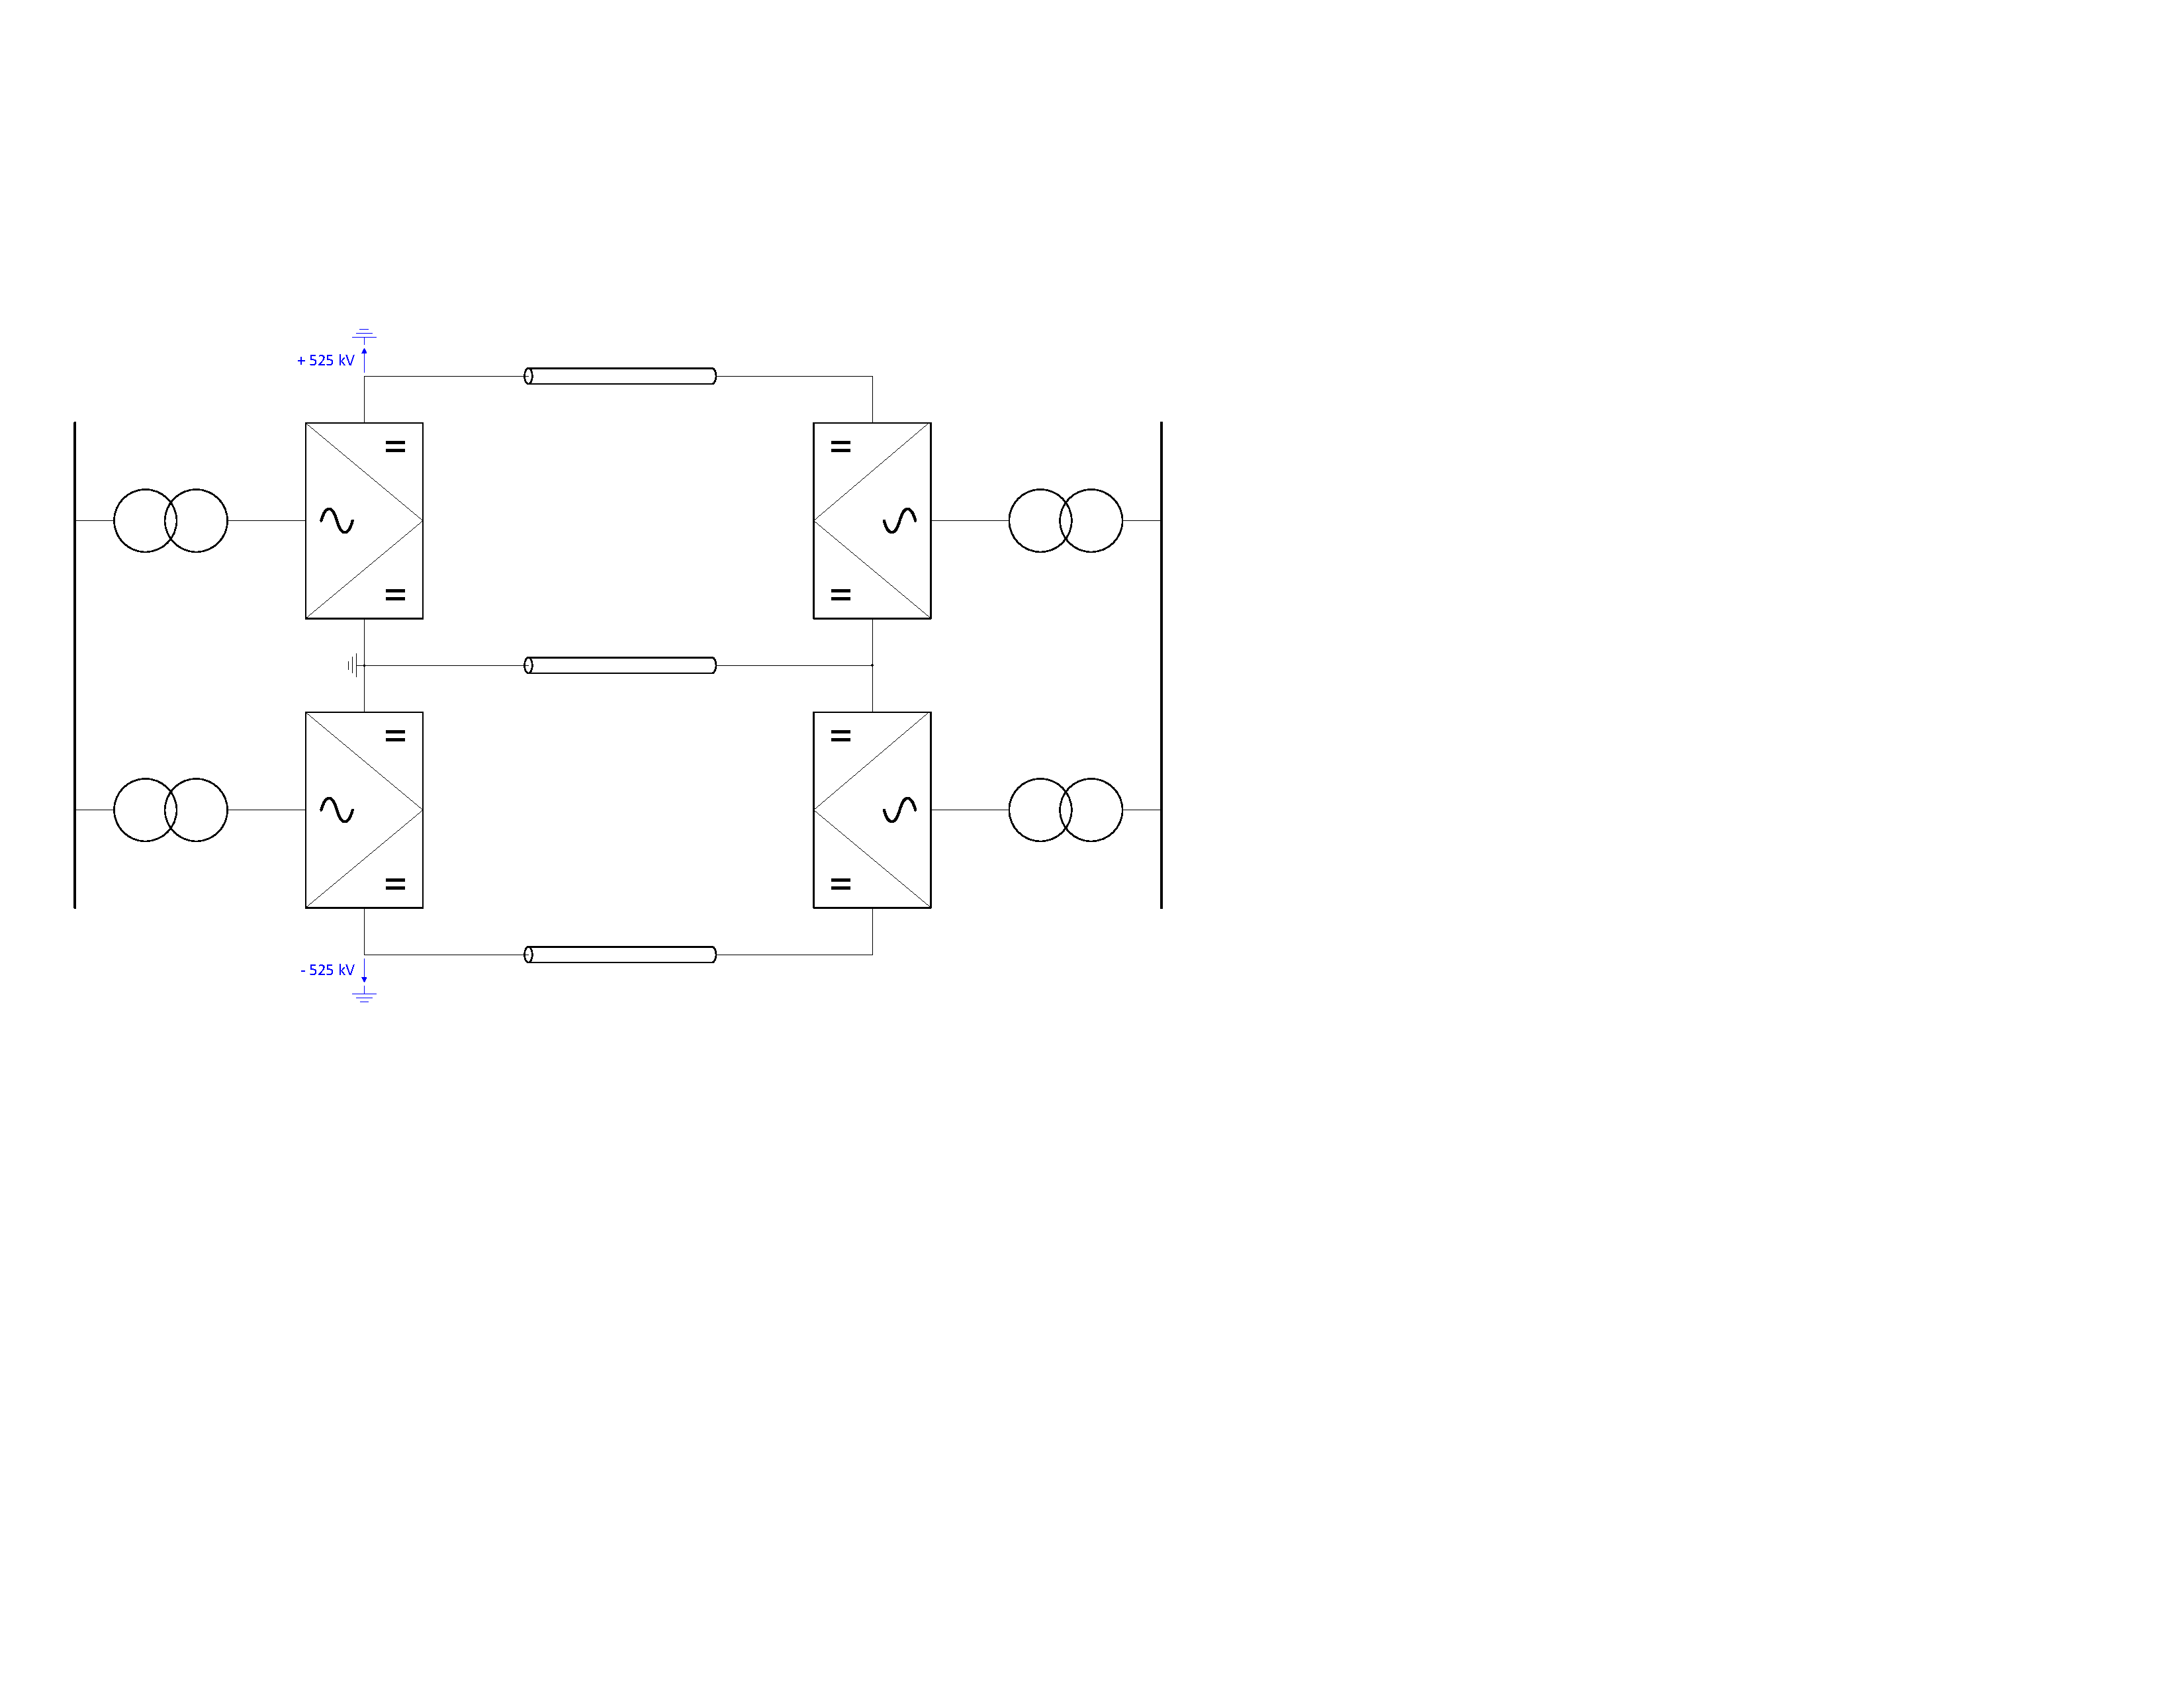
\includegraphics[width=0.7\linewidth]{fig/config_bip.pdf}
  \caption{Bipole with dedicated metallic return (BIP) configuration.}
  \label{fig:config-bip}
\end{figure}

\subsubsection{Scheme 2}
The anticipated transmission configuration for Scheme 2 is a symmetrical monopole with a DC voltage rating of $\pm$400\,kV (SMP, Figure~\ref{fig:config-smp}). 
The $\pm$400\,kV voltage selection is based on the Scheme 1 configuration, as this voltage level would allow to use the same converter configuration for both schemes. 
In case of BIP topology application for Scheme 1, a DC voltage of $\pm$320\,kV should be used.

\begin{figure}[htbp]
  \centering
  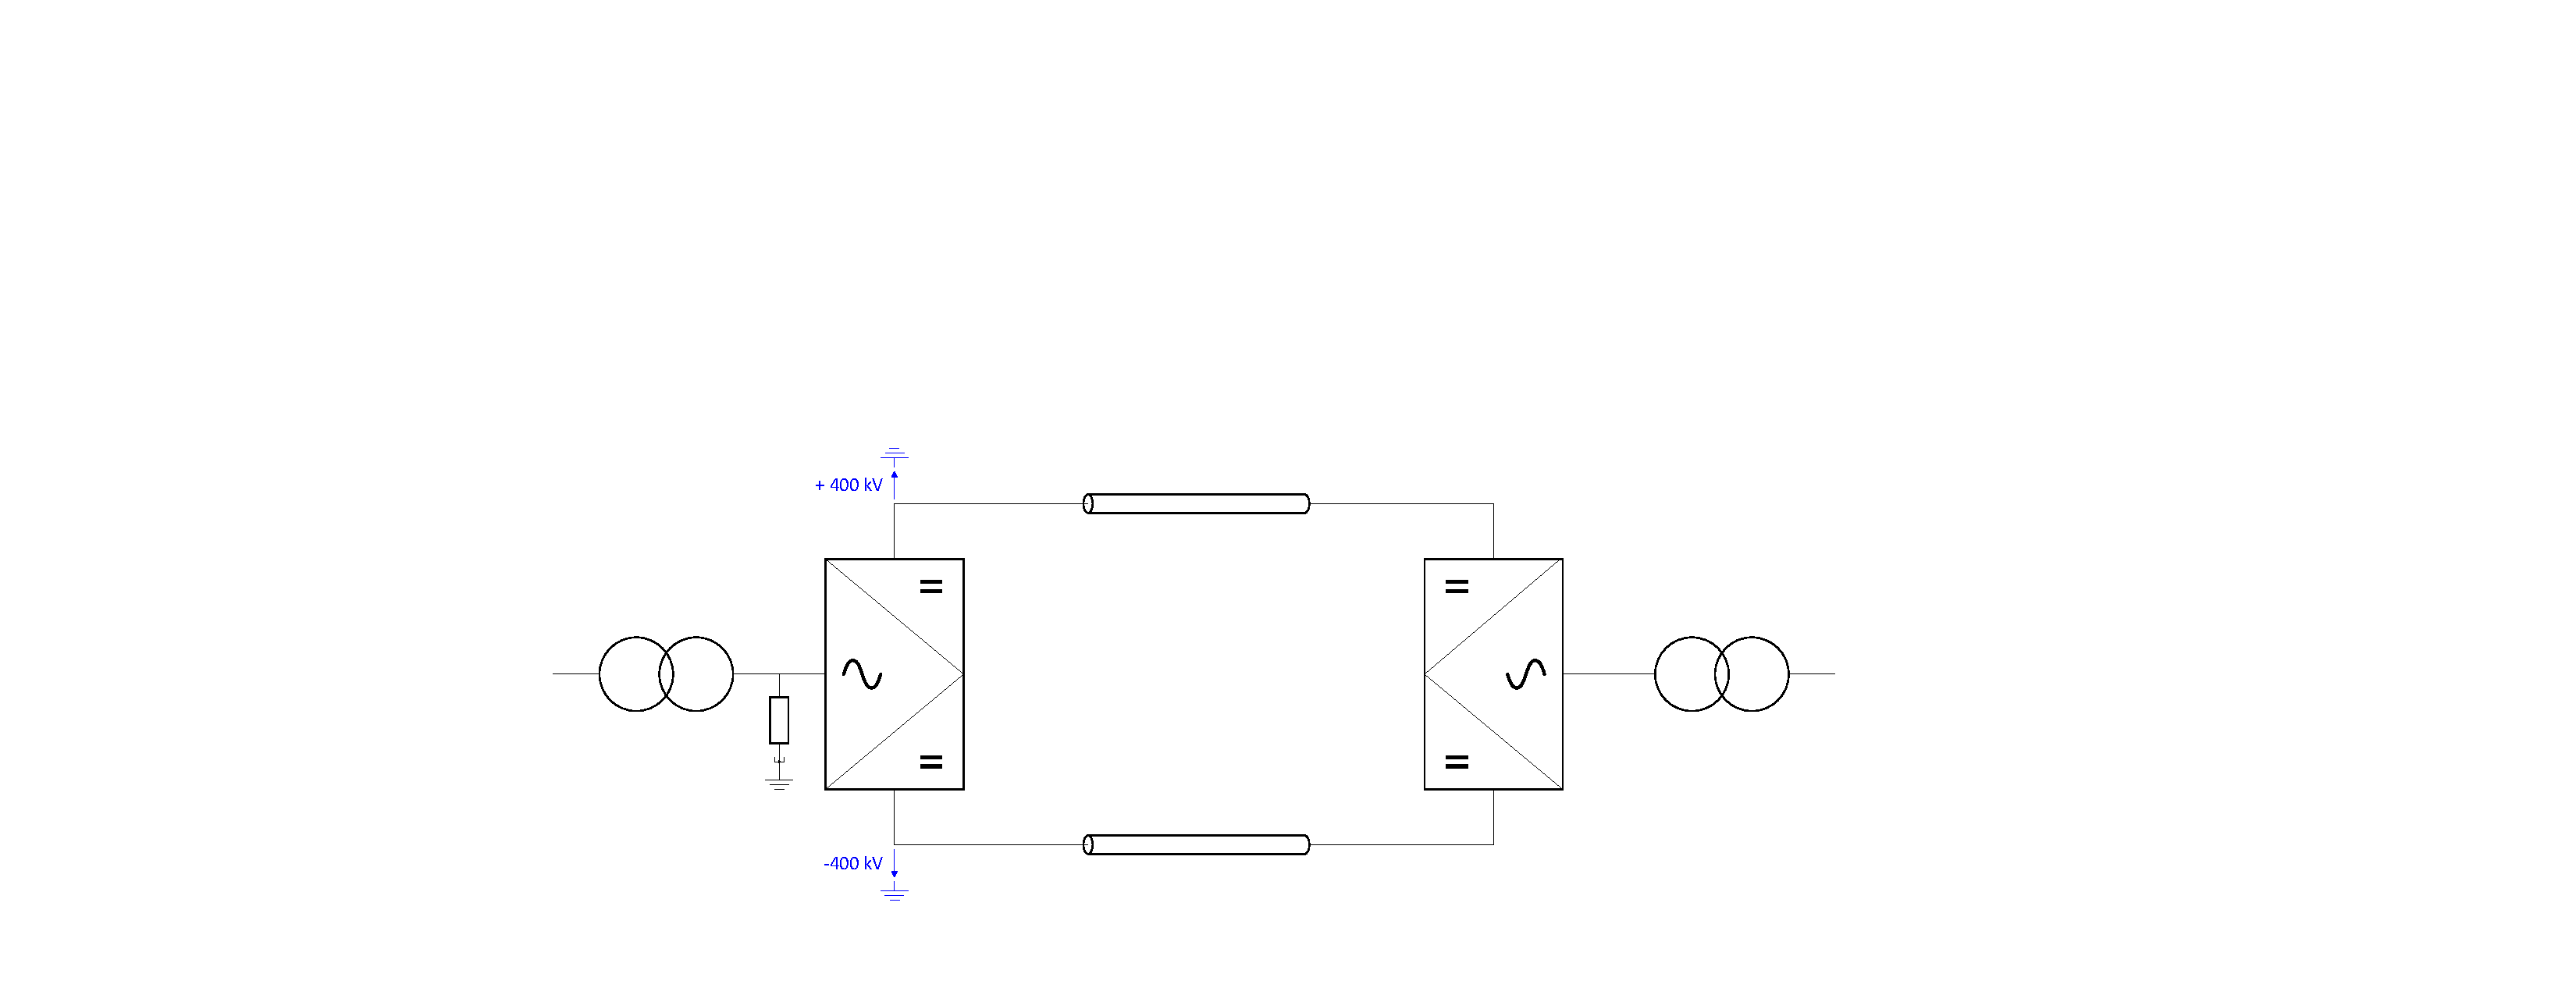
\includegraphics[width=0.7\linewidth]{fig/config_smp.pdf}
  \caption{Symmetrical monopole (SMP) configuration.}
  \label{fig:config-smp}
\end{figure}

\subsection{Generation at rectifier}
Organic Rankine Cycle (ORC) power generation systems will be used as the primary generation source. The individual generator units will be sized
at 40\,MW - 60\,MW.

American Terawatt will provide a generator-system equivalent to be used for EMT-type studies and performance verification, together with an RSCAD model for
hardware-in-the-loop (HIL) testing.

\subsection{Load at inverter}
The load connected to the HVDC system consists of data-center loads, which are characterized by power fluctuation. The system configuration 
will include compensation devices such as E-STATCOM or BESS which will compensate the power fluctuations. 

American Terawatt will provide a data-center load equivalent to be used for
EMT-type studies and performance verification, together with an RSCAD model for
hardware-in-the-loop (HIL) testing.
